% Full chain: pdflatex -> bibtex -> pdflatex -> pdflatex
\documentclass[11pt,en,cite=authoryear]{elegantpaper}

\title{Circulation theory of enzyme kinetics}

\author{Yuhao Jiang}
\date{\today}

%command
\usepackage{array}
\usepackage{amssymb}
\usepackage{graphicx,float,subfigure}
\usepackage{subfigure}
\usepackage[T1]{fontenc}
\usepackage[utf8]{inputenc}
\usepackage{mathtools}
\usepackage{bm}

\begin{document}

\maketitle
We consider the following m-step($n\ge 2$) enzyme kinetics model:
\begin{align} \label{eq:model}
    \bm{E + S \rightleftharpoons
    ES \rightleftharpoons
    EP_1 \rightleftharpoons
    EP_2 \rightleftharpoons
    \cdots
    EP_{m-2} \rightleftharpoons
    E + P}
\end{align}

where $\bm{E}$ is an enzyme turning the substrate $\bm{S}$ into the product $\bm{P}$. From the  perspective of a single enzyme molecule, this enzyme kinetics can be modeled as n-step Markov chain $(\xi_l)_{l\ge 0}$, with finite state space S defined on some space $(\Omega, \mathcal{F}, P)$. When $n=2$, this Markov chain only have two state $\bm{E}$ and $\bm{ES}$, we say that the state space $S=\{1, 2\}$.

\begin{definition}
    Let $\mathbb{Z}$ be the set of integers, and a periodic function $f$ which maps $\mathbb{Z}$ to S is called circuit function. If $s$ is the smallest positive integer which satisfied $f(n+s) = f(n)$ for $\forall n \in \mathbb{Z}$, then we called it the period of $f$.
\end{definition}

\begin{definition}
    Two circuit functions $f$ and $g$ in S are called equivalent if there exists some $m \in \mathbb{Z}$ such that $g(n) = f(n+m)$ for $\forall n \in \mathbb{Z}$.
\end{definition}
\begin{definition}
    For a circuit function $f$ in S with period $s$ that satisfies $f(1)=i_1$, $f(2)=i_2$, $f(3)=i_3$. The equivalence class that $f$ belongs is a cycle $c=(i_1, i_2, \dots i_s)$.
\end{definition}

Therefore, according to this definitions, $c_1 = (1, 2, 3), c_2 = (3, 1, 2)$ and $c_3 = (2, 3, 1)$ represent the same cycle. 
% So a cycle is also a equivalence class on the space of all circuit functions under the equivalence relation.

For presentation purposes, if the order sequence $i_1, i_2, \dots, i_s$ occurs in the cycle $c$ continuously, we denote that $[i_1, i_2, \dots, i_s] \in c$. Specially, if $[i_1] \in c$, the point $i_1$ occurrs in $c$, and $[i_1, i_2] \in c$ denotes the edge $i_1 i_2$ exists in the cycle $c$. 
For the cycle $c_1 = (1,2)$, we use $k_{12}$ to denote the number of cycle $c_1$.

\begin{definition}
    Let $\mathcal{C}_n(\omega)$ be the class of cycles occurring along the sample path $(\xi_l)_{l\ge 0}$ until time $n$. Then we use $\mathcal{C}_{\infty}$ to represent the limit of $\mathcal{C}_n$ as $n \rightarrow \infty$. This convergence has been proofed in \cite{jiang2004mathematical}.
\end{definition}

\begin{definition} %% follow Jia2016
    Let $k_{c, n}$ represent the number of time that cycle c is formed by a Markov chain up to time $n$. Then the sample circulation $J_{n}^c$ along cycle $c$ by time $t$ is defined as
    $$
    J_{n}^c = \frac{1}{n} k_{c, n} \quad \forall c \in \mathcal{C}_{\infty}
    $$
    and the circulation $w^c$ along cycle $c$ is a nonnegative real number defined as the following almost sure limit:
    $$
    w_c = \lim_{n \rightarrow \infty} J_{n}^c \quad \forall c \in \mathcal{C}_{\infty}, \quad a.s.
    $$
    which represents the number of times that cycle $c$ ic formed per unit time. Let $J_n = (J_n^c)_{c \in C_{\infty}}$ and $w =  (w_c)_{c \in C_{\infty}}$.
\end{definition}

For the enzyme kinetics model, if the state space $S=\{1, 2, \dots, m\}$, then $\mathcal{C}_{\infty}$ has $2m+2$ cycles, including $n$ 1-state cycles, $n$ two-state cycles and two n-state cycles

Let $|c|$ denotes the length of cycle $c$, and 
$E_m = \{\mu=(\mu_c)_{c\in \mathcal{C}_{\infty}} \in [0, 1]^r :\sum_{c \in \mathcal{C}_{\infty}} |c| \mu_c  = 1\}$ for m-state Markov chains, then the circulation distribution $w = (w_{c})_{c \in \mathcal{C}_{\infty}} \in E_m$.

\begin{definition}
    For m-state Markov chains, we say that $J_{n}^c$ satisfies a large deviation principle with rate $n$ and good rate function $I$ : $E_m \rightarrow [0, \infty]$ if:
    \begin{align}
        \lim_{n \rightarrow \infty} \frac{1}{n} \log \mathbb{P}(J_{n}^c = \nu_c , c \in \mathcal{C}_{\infty}) = - I(\nu), \quad \forall \nu \in E_m \rightarrow
    \end{align}
    where $\sum_{c \in \mathcal{C}_{\infty}} |c| \nu_c = 1$, 
    % $r$ is the size of set $\mathcal{C}_{\infty}$,
    and $\nu = (\nu_c)_{c \in \mathcal{C}_{\infty}} \in E_m$.
\end{definition}


\section{Large deviation of circulation for finite Markov chains}
\subsection{Large deviation of circulation for  finite state Markov chains}
\begin{figure}[h]
    \centering
    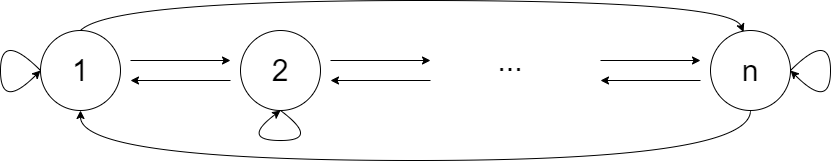
\includegraphics[scale=0.3]{chart/n-state2.png}
    \caption{m-state transition diagram}
\end{figure}
\begin{theorem}
    For the m-state Markov chains, the good rate function is
    \begin{align*}
        I_m^c(\nu)
        &= [h(\nu_{12}+\nu_{1 m}+\nu^+ +\nu^-) - h(\nu_{12}) - h(\nu_{1m})+
        h(\nu^+) + h(\nu^-)]
        + \sum_{i \in S} [h(\nu^i) - h(\nu^i-\nu_i)]\\
        &+ \max_{\nu^+_{ij} + \nu^-_{ij} = \nu_{ij}, i\neq 1, j\neq m} \biggl\{
        [h(\nu_{12}+\nu^+_{23}+\nu^+) - h(\nu^+_{23}) - h(\nu_{12}+\nu^+)]\\
        &+[h(\nu^+_{34}+\nu^+_{23}+\nu^+) - h(\mu^+_{34}) - h(\nu^+_{23}+\nu^)]+
        \dots +\\
        &+[h(\nu^+_{m-1,m} + \nu^+_{m-2,m-1} + \nu^+) - h((\nu^+_{m-1,m})- h(\nu^+_{m-2,m-1} + \nu^+)] \\
        &+ [h(\nu_{1m}+ \nu^{-}_{m-1,m}+ \nu^-) -h(\nu^-_{m-1,m}) -h(\nu_{1m}+\nu^-)]\\
        &+ [h(\nu^-_{m-1,m} +\nu^-_{m-2,m-1} +\nu^-) -h(\nu^-_{m-2,m-1}) -h(\nu^-_{m-1,m} +\nu^-)]\\
        &+ \dots +
        + h(\nu^-_{23}+\nu^-_{34}+\nu^-) - h(\nu^-_{23}) -h(\nu^-_{34}+\nu^-)\biggr\}
        + \sum_{i,j} (\sum_{c \ni [i,j]}\nu_c) \log p_{ij}
    \end{align*}
\end{theorem}
\begin{proof}
    
\end{proof}
\end{document}